% GNUPLOT: LaTeX picture with Postscript
\begingroup
  \makeatletter
  \providecommand\color[2][]{%
    \GenericError{(gnuplot) \space\space\space\@spaces}{%
      Package color not loaded in conjunction with
      terminal option `colourtext'%
    }{See the gnuplot documentation for explanation.%
    }{Either use 'blacktext' in gnuplot or load the package
      color.sty in LaTeX.}%
    \renewcommand\color[2][]{}%
  }%
  \providecommand\includegraphics[2][]{%
    \GenericError{(gnuplot) \space\space\space\@spaces}{%
      Package graphicx or graphics not loaded%
    }{See the gnuplot documentation for explanation.%
    }{The gnuplot epslatex terminal needs graphicx.sty or graphics.sty.}%
    \renewcommand\includegraphics[2][]{}%
  }%
  \providecommand\rotatebox[2]{#2}%
  \@ifundefined{ifGPcolor}{%
    \newif\ifGPcolor
    \GPcolortrue
  }{}%
  \@ifundefined{ifGPblacktext}{%
    \newif\ifGPblacktext
    \GPblacktexttrue
  }{}%
  % define a \g@addto@macro without @ in the name:
  \let\gplgaddtomacro\g@addto@macro
  % define empty templates for all commands taking text:
  \gdef\gplbacktext{}%
  \gdef\gplfronttext{}%
  \makeatother
  \ifGPblacktext
    % no textcolor at all
    \def\colorrgb#1{}%
    \def\colorgray#1{}%
  \else
    % gray or color?
    \ifGPcolor
      \def\colorrgb#1{\color[rgb]{#1}}%
      \def\colorgray#1{\color[gray]{#1}}%
      \expandafter\def\csname LTw\endcsname{\color{white}}%
      \expandafter\def\csname LTb\endcsname{\color{black}}%
      \expandafter\def\csname LTa\endcsname{\color{black}}%
      \expandafter\def\csname LT0\endcsname{\color[rgb]{1,0,0}}%
      \expandafter\def\csname LT1\endcsname{\color[rgb]{0,1,0}}%
      \expandafter\def\csname LT2\endcsname{\color[rgb]{0,0,1}}%
      \expandafter\def\csname LT3\endcsname{\color[rgb]{1,0,1}}%
      \expandafter\def\csname LT4\endcsname{\color[rgb]{0,1,1}}%
      \expandafter\def\csname LT5\endcsname{\color[rgb]{1,1,0}}%
      \expandafter\def\csname LT6\endcsname{\color[rgb]{0,0,0}}%
      \expandafter\def\csname LT7\endcsname{\color[rgb]{1,0.3,0}}%
      \expandafter\def\csname LT8\endcsname{\color[rgb]{0.5,0.5,0.5}}%
    \else
      % gray
      \def\colorrgb#1{\color{black}}%
      \def\colorgray#1{\color[gray]{#1}}%
      \expandafter\def\csname LTw\endcsname{\color{white}}%
      \expandafter\def\csname LTb\endcsname{\color{black}}%
      \expandafter\def\csname LTa\endcsname{\color{black}}%
      \expandafter\def\csname LT0\endcsname{\color{black}}%
      \expandafter\def\csname LT1\endcsname{\color{black}}%
      \expandafter\def\csname LT2\endcsname{\color{black}}%
      \expandafter\def\csname LT3\endcsname{\color{black}}%
      \expandafter\def\csname LT4\endcsname{\color{black}}%
      \expandafter\def\csname LT5\endcsname{\color{black}}%
      \expandafter\def\csname LT6\endcsname{\color{black}}%
      \expandafter\def\csname LT7\endcsname{\color{black}}%
      \expandafter\def\csname LT8\endcsname{\color{black}}%
    \fi
  \fi
    \setlength{\unitlength}{0.0500bp}%
    \ifx\gptboxheight\undefined%
      \newlength{\gptboxheight}%
      \newlength{\gptboxwidth}%
      \newsavebox{\gptboxtext}%
    \fi%
    \setlength{\fboxrule}{0.5pt}%
    \setlength{\fboxsep}{1pt}%
    \definecolor{tbcol}{rgb}{1,1,1}%
\begin{picture}(4020.00,4160.00)%
    \gplgaddtomacro\gplbacktext{%
      \csname LTb\endcsname%%
      \put(734,386){\makebox(0,0){\strut{}$-150$}}%
      \csname LTb\endcsname%%
      \put(1157,386){\makebox(0,0){\strut{}$-100$}}%
      \csname LTb\endcsname%%
      \put(1581,386){\makebox(0,0){\strut{}$-50$}}%
      \csname LTb\endcsname%%
      \put(2004,386){\makebox(0,0){\strut{}$0$}}%
      \csname LTb\endcsname%%
      \put(2428,386){\makebox(0,0){\strut{}$50$}}%
      \csname LTb\endcsname%%
      \put(2851,386){\makebox(0,0){\strut{}$100$}}%
      \csname LTb\endcsname%%
      \put(3275,386){\makebox(0,0){\strut{}$150$}}%
    }%
    \gplgaddtomacro\gplfronttext{%
      \csname LTb\endcsname%%
      \put(2004,123){\makebox(0,0){\normalsize $\Phi$}}%
      \csname LTb\endcsname%%
      \put(2423,961){\rotatebox{43.00}{\makebox(0,0){\strut{}\textcolor{black}{\footnotesize 3.0}}}}%
      \csname LTb\endcsname%%
      \put(2242,1983){\rotatebox{129.00}{\makebox(0,0){\strut{}\textcolor{black}{\footnotesize 2.5}}}}%
      \csname LTb\endcsname%%
      \put(1050,3244){\rotatebox{-72.00}{\makebox(0,0){\strut{}\textcolor{black}{\footnotesize 2.5}}}}%
      \csname LTb\endcsname%%
      \put(2089,3450){\makebox(0,0){\strut{}\textcolor{black}{\footnotesize 2.5}}}%
      \csname LTb\endcsname%%
      \put(1215,726){\rotatebox{40.00}{\makebox(0,0){\strut{}\textcolor{black}{\footnotesize 2.5}}}}%
      \csname LTb\endcsname%%
      \put(2273,1132){\rotatebox{42.00}{\makebox(0,0){\strut{}\textcolor{black}{\footnotesize 2.5}}}}%
      \csname LTb\endcsname%%
      \put(3284,1547){\rotatebox{-22.00}{\makebox(0,0){\strut{}\textcolor{black}{\footnotesize 2.5}}}}%
      \csname LTb\endcsname%%
      \put(881,3459){\rotatebox{-108.00}{\makebox(0,0){\strut{}\textcolor{black}{\footnotesize 2.0}}}}%
      \csname LTb\endcsname%%
      \put(1261,2785){\rotatebox{-4.00}{\makebox(0,0){\strut{}\textcolor{black}{\footnotesize 2.0}}}}%
      \csname LTb\endcsname%%
      \put(2288,3240){\rotatebox{-5.00}{\makebox(0,0){\strut{}\textcolor{black}{\footnotesize 2.0}}}}%
      \csname LTb\endcsname%%
      \put(1813,1009){\rotatebox{24.00}{\makebox(0,0){\strut{}\textcolor{black}{\footnotesize 2.0}}}}%
      \csname LTb\endcsname%%
      \put(1966,1768){\rotatebox{145.00}{\makebox(0,0){\strut{}\textcolor{black}{\footnotesize 2.0}}}}%
      \csname LTb\endcsname%%
      \put(1797,2466){\rotatebox{-23.00}{\makebox(0,0){\strut{}\textcolor{black}{\footnotesize 2.0}}}}%
      \csname LTb\endcsname%%
      \put(2702,1868){\rotatebox{-19.00}{\makebox(0,0){\strut{}\textcolor{black}{\footnotesize 2.0}}}}%
      \csname LTb\endcsname%%
      \put(697,2110){\rotatebox{50.00}{\makebox(0,0){\strut{}\textcolor{black}{\footnotesize 1.5}}}}%
      \csname LTb\endcsname%%
      \put(1552,1927){\rotatebox{-50.00}{\makebox(0,0){\strut{}\textcolor{black}{\footnotesize 1.5}}}}%
      \csname LTb\endcsname%%
      \put(1614,1148){\rotatebox{-173.00}{\makebox(0,0){\strut{}\textcolor{black}{\footnotesize 1.5}}}}%
      \csname LTb\endcsname%%
      \put(2795,3106){\rotatebox{-155.00}{\makebox(0,0){\strut{}\textcolor{black}{\footnotesize 1.5}}}}%
      \csname LTb\endcsname%%
      \put(1951,2630){\rotatebox{-36.00}{\makebox(0,0){\strut{}\textcolor{black}{\footnotesize 1.5}}}}%
      \csname LTb\endcsname%%
      \put(2931,2166){\rotatebox{16.00}{\makebox(0,0){\strut{}\textcolor{black}{\footnotesize 1.5}}}}%
      \csname LTb\endcsname%%
      \put(596,884){\rotatebox{75.00}{\makebox(0,0){\strut{}\textcolor{black}{\footnotesize 1.0}}}}%
      \csname LTb\endcsname%%
      \put(970,1975){\rotatebox{14.00}{\makebox(0,0){\strut{}\textcolor{black}{\footnotesize 1.0}}}}%
      \csname LTb\endcsname%%
      \put(1322,1277){\rotatebox{-156.00}{\makebox(0,0){\strut{}\textcolor{black}{\footnotesize 1.0}}}}%
      \csname LTb\endcsname%%
      \put(2732,2908){\rotatebox{-158.00}{\makebox(0,0){\strut{}\textcolor{black}{\footnotesize 1.0}}}}%
      \csname LTb\endcsname%%
      \put(2947,2371){\rotatebox{11.00}{\makebox(0,0){\strut{}\textcolor{black}{\footnotesize 1.0}}}}%
      \csname LTb\endcsname%%
      \put(1234,1635){\rotatebox{116.00}{\makebox(0,0){\strut{}\textcolor{black}{\footnotesize 0.5}}}}%
      \csname LTb\endcsname%%
      \put(2004,3876){\makebox(0,0){Dipole Strength (D)}}%
    }%
    \gplbacktext
    \put(0,0){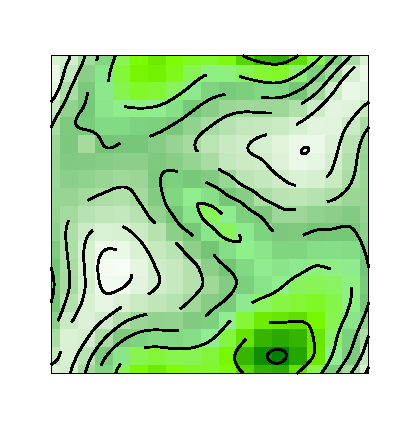
\includegraphics[width={201.00bp},height={208.00bp}]{Q1_d}}%
    \gplfronttext
  \end{picture}%
\endgroup
